\label{Definitions}
\section{Introduction}

The first definition of a cograph was introduced by Seinsche in 1974 \cite{Seinsche1974OnAP}. Since then, the class of cographs has been actively studied. Many algorithms for recognizing and calculating their properties have been invented.

The most common definition of cographs is graphs do not contain $P_4$ as an induced subgraph. This article implements a cograph recognition algorithm using factorizing permutations. The idea of the algorithm was conceived by Michel Habib and Christophe Paul \cite{HABIB2005183}. The algorithm consists of two parts. In the first part, a permutation of the graph's vertices that meets certain conditions is constructed. For this, vertex partitioning and part refinement are used. The second part of the algorithm is testing the obtained permutation of the graph. During testing, some vertices are removed from the permutation. If at the end of the testing there is exactly one vertex left in the permutation, then the graph is a cograph. Both parts of the algorithm work in linear time.

It is a well-known fact that for a cograph, there exists a canonical tree called a cotree \cite{CORNEIL1981163}. For constructing a cotree we used the algorithm described by Michel Habib and Christophe Paul. It is based on the vertex removal order obtained in the second part of the recognition algorithm. This cotree construction algorithm works in linear time.

Using a cotree corresponding to a cograph, we can solve in linear time problems that are NP-complete in the general case. These solutions are often achieved using dynamic programming. This paper presents an algorithm for finding the pathwidth and treewidth of a cograph. The algorithm was introduced by Hans Bodlaender and Rolf Möhring \cite{Sumner1974DaceyG}. Algorithms for finding the maximum clique and the maximum independent set were invented by Derek Corneil, Helmut Lerchs, and  Lauren Stewart \cite{CORNEIL1981163}. The general scheme for calculating properties of cograph is demonstrated on the example of a cograph coloring algorithm. 

There are many problems with polynomial solutions in the class of cographs, in addition to those mentioned. For example: algorithm for simple max-cut \cite{Bodlaender1994OnTC}  or hamiltonicity \cite{corneil_lerchs_stewart_81}.
But not every NP-complete problem in the general case has a polynomial solution for the class of cographs. For example, problems such as determining whether a given cograph $G$ is a subgraph of a given cograph $H$ \cite{damaschke_91}, computing the achromatic number \cite{Bodlaender1989AchromaticNI}, or list coloring \cite{Jansen1992GeneralizedCF} for cographs remain NP-hard.

Many problems about whether a graph can be transformed into a cograph by deleting some edges or vertices are FPT-complete. 
For example:
\begin{itemize}
    \item $k$-edge-deletion to cographs in $O(2.562^k \cdot (m + n))$ time \cite{nastos_gao_10}.
    \item $k$-vertex-deletion algorithm in $O(3.303^k \cdot (m +n))$ time \cite{nastos_gao_10}.
    \item $k$-edge-edited to cographs in $O(4.612^k \cdot (m+n))$ time \cite{Liu2012ComplexityAP}.
    \item a graph can be made into a cograph by deleting at most $i$ vertices, at most $j$ edges is fixed parameter tractable with respect to $i$ and $j$ \cite{Cai1996FixedParameterTO}.
\end{itemize}


\Cref{Definitions} presents the main definitions and the structure of cograph and cotree. \Cref{Algorithm} is dedicated to the cograph recognition algorithm. 
In \Cref{Properties} there are present algorithms for finding the maximum clique, the maximum independent set, and the graph coloring. \Cref{Properties} also presents algorithms for finding pathwidth and treewidth. The description of the code and testing can be found in \Cref{last}.

\section{Basic definitions of graph theory}


Definitions of graph theory are taken from the books by Béla Bollobás, “Modern Graph Theory” \cite{Bollobs2002ModernGT}. 


Throughout this paper we consider only finite undirected simple graphs.

\begin{definition}[Graph]
  A \emph{graph} $G$ is an ordered pair of disjoint sets $(V, E)$ such that $E$ is the subset of the set $V \choose 2$ of unordered pairs of $V$.
\end{definition}

We call the graph trivial if it consists at most one vertex.

\begin{definition}[Subgraph]
  A graph $G' = (V', E')$ is a \emph{subgraph} of $G = (V, E)$ if $V' \subseteq V$ and $E' \subseteq E$.
\end{definition}

\begin{definition}[Induced subgraph]
  If $G' = (V', E')$ is a subgraph of $G$ and  forall $x$ and $y$ $\in V$ it holds that both  $ V' \subseteq V$ and $\{x,y\} \in E'$ if and only if  $\{x,y\} \in E'$ , then $G'$ is an \emph{induced subgraph} of $G$ and is denoted $G[V']$.
\end{definition}

\begin{definition}[$H$-free graph]
    For graphs $H$ and $G$, we say that $G$ is \emph{$H$-free} if and only if for every induced subgraph $G'$ of $G$, $G' \ne H$.
\end{definition}


\begin{definition}[Path]
  A \emph{path} is a graph $P=(V,E)$ of the form \[ V = \{x_1, x_2, \ldots, x_m\},\quad E = \{ \{x_1,x_2\}, \{x_2,x_3\} , \ldots, \{x_{m-1},x_m\} \} \] where for all distinct $i$ and $j \in V$ we have $x_i \ne x_j $

  This \emph{path} $P$ is usually denoted by $(x_1, x_2, \ldots, x_m)$.
\end{definition}

 We call a $P_i$ a path consisting of i vertices.

\begin{definition}[Cycle]
  If a graph $W =(V,E)$ where $V=(x_0, x_1 \ldots , x_l)$ and \[E= \bigcup_{i=0}^{l-1} \{x_i,x_{i+1} \} \] is such that $l \geq 3$, $x_0 = x_l$, and for all distinct $i,j \in [0,l-1]$ it hold that  $x_i \neq x_j$ , then $W$ is called a \emph{cycle}.
\end{definition}

\begin{definition}[Connected graph]
     A graph $G=(V,E)$ is \emph{connected} if for every pair $(x,y) \subseteq V$ of distinct vertices, there is a \emph{path} from $x$ to $y$.
\end{definition}

\begin{definition}[Forest, Tree]
    A graph without any cycles is a \emph{forest}, or equivalently an acyclic graph. A \emph{tree} is a connected forest.
\end{definition}

\begin{definition}[Neighbours, $N(x)$]
    For a given vertex x in graph $G=(V,E)$, let $N(x)$ denote the neighborhood of vertex, that is $\{ y \in V \colon \{x,y\} \in E  \}$. 
\end{definition}

Let us define the set $\bar{N}(x)$ as the set of all non-neighbors of vertex $x$ in the graph that is $\{ y \in V \colon y \notin N(x) \}$.

\begin{definition}[Chromatic number, $\chi(G)$]
    The chromatic number $\chi(G)$ of a graph $G=(V,E)$ is the smallest number of colors for $V$ so that adjacent vertices are colored differently. 
\end{definition}
Here we introduce key definitions necessary for the analysis of trees and, in particular, cotrees.

\begin{definition}[True twins and False twins]
Vertices $x,y$ are called \emph{true twins} (\emph{false twins}) if $N(x) \cup \{y\} = N(y) \cup \{x\}$ (respectively, if $N(x) = N(y)$).
\end{definition}

\begin{definition}[Rooted tree]
    A \emph{rooted tree} is a tree in which a special labeled node is singled out. This node is called the \emph{root}.
\end{definition}

\begin{definition}[Depth]
The \emph{depth} of vertex $v$ in a rooted tree $T$ is the distance between $v$ and root of $T$. 
\end{definition}

\begin{definition}[Child]
    In a rooted tree $T=(V,E)$, a vertex $y$ is a \emph{Child} of vertex $x$ if and only if $\{x,y\} \in E$ and vertex $x$ belongs to the path from vertex $y$ to the root of the tree.
\end{definition}

\begin{definition}[Descendants, $D(x)$]
For a given vertex x in graph $G=(V,E)$, let $D(x)$ denote the set of descendants of a vertex, that is, $D(x)=\{y \in V \colon $  vertex $x$ belongs to the path from vertex $y$ to the root of the tree $ \}$
\end{definition}

\begin{definition}[Subtree]
    In a tree $T$ the induced subgraph of a vertex $x$ and the set of all its descendants is called the \emph{subtree} of vertex $x$.
\end{definition}


We denote the subtree of vertex $x$ in tree $T$ as $T_x$.


\begin{definition}[Diameter]
    A \emph{diameter} of graph $G$ is denoted by $diam(G)$ and is maximum distance between any two vertices in $G$. 
\end{definition}

\begin{definition}[Least Common Ancestor, LCA]
The \emph{least common ancestor} of two nodes $x$ and $y$ in a tree $T$ is the vertex with maximum depth that has both $x$ and $y$ as descendants.
\end{definition}

\begin{definition}[Complement]
  For a graph $G = (V, E)$ the \emph{complement} of $G$ is a graph $\bar{G} = (V, {V \choose 2} \setminus E)$; thus, two vertices are adjacent in $\bar{G}$ if and only if they are not adjacent in $G$.
\end{definition}



\section{Cograph}
Definitions are taken from the article ``A simple linear time algorithm for cograph recognition'' \cite{HABIB2005183}.

There are many different definitions of the class of cographs. The \Cref{Fundamental theorem} on their equivalence was proven in the paper ``Complement reducible graphs'' \cite{CORNEIL1981163}.

\begin{theorem}[Theorem 2 in \cite{CORNEIL1981163}]
Given a graph $G$, the foIlowing statements are equivalent:
\begin{enumerate}
    \item  $G$ is a cograph.
    \item  Any nontrivial subgraph of $G$ has at least one pair of twins.
    \item $G$ does not contain $P_4$ as a subgraph.
    \item The complement of any nontrivial connected subgraph of G is disconnected.
\end{enumerate}
\label{Fundamental theorem}
\end{theorem}
The second statement of this theorem is proven below.

We also use the definition of a cograph through parallel and series composition operations.

\begin{definition}[Parallel composition, $\cup$]
    A \emph{parallel composition} of two graphs $G=(V_1,E_1)$ and $H=(V_2,E_2)$ is denoted by $G \cup H = (V_1 \cup V_2, E_1 \cup E_2)$.
\end{definition}

\begin{definition}[Series composition, $\times$]
A graph $G$ is the \emph{series composition} of $G_1$ and $G_2$ if $V=  V_1 \cup V_2$ and $E=E_1\cup E_2 \cup \{ \{x_1,x_2\}  \colon x_1 \in E_1$ and $x_2 \in E_2  \}$
\end{definition}
\begin{theorem}[Definition 1 in \cite{HABIB2005183}] 
     A graph $G=(V,E)$ is a cograph if and only if one of the following
conditions holds:
\begin{itemize}
    \item $ |V| = 1$
    \item  There are cographs $G_1, \dots, G_k$ such that $G_1 \cup G_2 \cup \dots \cup G_k=G$.
    \item There are cographs $G_1, \dots, G_k$ such that $G_1 \times G_2 \times \dots \times G_k=G$.
\end{itemize}
\end{theorem}

Every graph can be represented as a formula using parallel compositions and series compositions of single-vertex graphs, often in multiple ways. This formula can be depicted as a tree, where each leaf corresponds to a single-vertex graph and each internal node corresponds to a parallel or series composition . In other words, each subtree of a tree corresponds to a certain cograph, and the internal nodes of the tree determine the order and type of compositions. Such a tree is called a cotree. In a canonical cotree, there are no adjacent nodes of the same type. See on an example of a graph and its corresponding cotree in \Cref{fig:Example}.

\begin{figure}
\centering
    \begin{subfigure}[b]{0.35\textwidth}
    \centering
    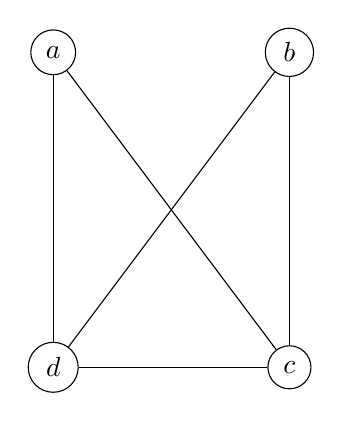
\begin{tikzpicture}[every node/.style={circle,draw,minimum size=5mm}]
  \node (a) at (0, 4) {$a$};
  \node (b) at (3, 4) {$b$};
  \node (c) at (3, 0) {$c$};
  \node (d) at (0, 0) {$d$};


  \draw (a) -- (c);
  \draw (a) -- (d);
  \draw (b) -- (c);
  \draw (b) -- (d);
  \draw (c) -- (d);
  
\end{tikzpicture}

    \caption{Graph and it's cotree (left)}
    \label{fig:An example cograph}
    \end{subfigure}
    \qquad
    \begin{subfigure}[b]{0.55\textwidth}
    \centering
    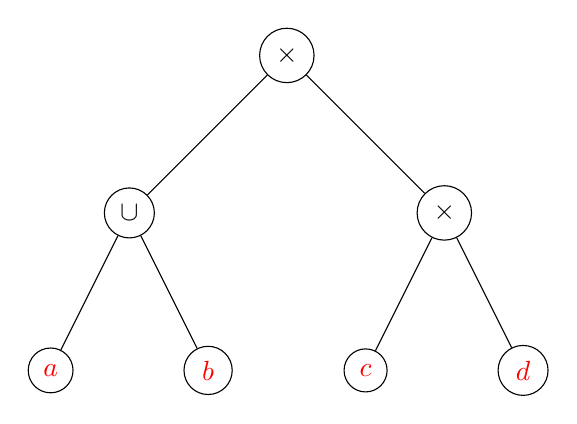
\begin{tikzpicture}[every node/.style={circle,draw,minimum size=5mm},level distance=2cm,
  level 1/.style={sibling distance=4cm},
  level 2/.style={sibling distance=2cm}
  ]
    
    \node {$\times$}
        child { node {$\cup$}
                child { node {\textcolor{red}{$a$} }}
                child { node {\textcolor{red}{$b$}} }
        }
        child{ node {$\times$}
                child { node {\textcolor{red}{$c$} }}
                child { node {\textcolor{red}{$d$}} }
        }
        ;
\end{tikzpicture}
    \caption{Graph and it's cotree (right)}
    \label{fig:An example cotree}
    \end{subfigure}
    \label{fig:Example}
    \caption{Example}
\end{figure}

The following fact follows from the construction of the cotree:

\begin{remark}
In a cograph, two vertices $x$ and $y$ are adjacent if and only if their least common ancestor in the cotree is a series node.
\label{Ancestors remark}
\end{remark}

For example, in the cograph shown in the \Cref{fig:An example cograph}, vertices $a$ and $d$ are adjacent, and their least common ancestor in the cotree is a series node. On the other hand, vertices $a$ and $b$ are not adjacent, and their least common ancestor is a parallel node.

\begin{theorem}[Lemma 1 in \cite{CORNEIL1981163}]
    Every subgraph of a cograph is a cograph.
\end{theorem}

\begin{proof}
    To prove this, it is sufficient to show that a cograph remains a cograph even after the removal of any vertex. Let $T$ be the cotree corresponding to the cograph $G$. Let $G_1$ be the induced subgraph of $G$ without vertex $x$. We construct the cotree $T_1$ corresponding to the graph $G_1$.
Suppose vertex $y$ is the parent of vertex $x$ in tree $T$. If vertex $y$ had more than two children, then tree $T_1$ is obtained from tree $T$ by removing vertex $x$ and the edge $\{x,y\}$.
Otherwise, let $z$ be the second child of vertex $y$, and let $w$ be the parent of vertex $y$. Tree $T_1$ is obtained from tree $T$ by removing vertices $x$ and $y$ and all edges connected to them, and by adding the edge $\{w,z\}$. Thus, for any vertex $x$ and any cotree $T$, exists a cotree $T_1$. Therefore, graph $G_1$ is a cograph, and consequently, any induced subgraph of a cograph is also a cograph.
\end{proof}

Knowing this fact, we can prove statement 2 of \Cref{Fundamental theorem}. A graph is a cograph if and only if any of its nontrivial subgraphs has a pair of twin vertices.
Every nontrivial subgraph of a cograph is a cograph. Therefore, a cotree exists for any subgraph. In any nontrivial tree, there are two sibling vertices. If the vertices are siblings in the cotree, then they are twins in the cograph. If there are two twin vertices in every nontrivial subgraph of a graph, a cotree can be constructed for such a graph. Hence, this graph is a cograph.
A more detailed proof of these facts is in the \cref{Constructing the cotree}.

From \Cref{Ancestors remark}, it follows that for each vertex $n$ and for each vertex in $T_n$, the set of neighbors outside $T_n$ is the same because least common ancestor is the same for any vertex $x$ in $T$ and a fixed vertex $y$ not in $T_n$ .  

A set of vertices in the graph that possesses this property is called a module.Formally:
\begin{definition} [Module Definition 1 in \cite{HABIB2005183}]
For a graph $G=(V,E)$. A set of vertices $M \subseteq V$ is a \emph{module} if and only if for any $z$ and $t \in$  $M$ it holds that $N(z)/M=N(t)/M$.
\end{definition}

\begin{definition} [Strong module Definition 1 in \cite{HABIB2005183}]
A module $M$ is a strong \emph{module} if and only if for any module $M_1$ it holds that either $ M_1 \subseteq M$ or $ M \subseteq M_1$ or $M_1 \cap M = \emptyset$.
\end{definition}

If the set of vertices $M$ of the cograph is a strong module and is not the set of leaves of some subtree of the cotree, then exist a subtree of the cotree $T_r$ and $T_r \cap M \neq T_r$, $T_r \cap M \neq M$, $T_r \cap M \neq \omega$. This, for example, holds if $r$ is vertex from $M$ with maximum depth such that it has a child $y \notin M$.

Consequently:
\begin{remark}[Remark 6 in \cite{HABIB2005183}] 
    For any strong module $M$, there is an internal node $n$ of the cotree $T$ such that $M$ is exactly the set of leaves of $T_n$.
\end{remark}

The first step of the cograph recognition algorithm is the construction of the factorizing permutation of the graph's vertices. Let us define it as follows :

\begin{definition}[Definition 7 in \cite{HABIB2005183}]
    A factorizing permutation of a graph $G =(V,E)$ is a permutation $\sigma$ of the vertex set $V$ such that the vertices of any strong module of $G$ appears consecutively in $\sigma$.
\end{definition}

Factorizing permutations are convenient to use due to the existing bijection between them and the planar representations of cotrees.

\begin{theorem}[Lemma 9 in \cite{HABIB2005183}]
    For each planar representation of a cotree, the leaves in the order of a left-to-right depth-first search forms a factorizing permutation. This is because the leaves of each subtree appear consecutively in the formed permutation. Consequently, the vertices of each strong module appear consecutively.

The existence of a unique planar representation of a cotree for each factorizing permutation is proven by induction on the size of the permutation.
\end{theorem}

\begin{definition}[Definition 8 in \cite{HABIB2005183}]
    Let $x, y, z$ be three distinct vertices in a graph $G=(V,E)$. Then $x$ separates $y$ and $z$ if either $\{x,y\} \in E $ and $\{x,z\} \notin E$ or $\{x,y\} \notin E $ and $\{x,z\} \in E$.
\end{definition}


Now, using the properties of the cotree, we derive an important fact for the cograph recognition algorithm. To do this, let us introduce another definition :

\begin{remark}[Corollary 11 in \cite{HABIB2005183}]
    Let $x, y, z$ be distinct vertices appearing in that order in a factorizing permutation $\sigma$ such that $\{x,y\} \notin E$ and $\{y,z\} \in E$. Then $\{x,z\} \in E $ if and only if LCA$(x,y)$ is a descendant of LCA$(y,z)$.
    \label{Corollary 11}
\end{remark}

\begin{figure}
\centering
     \begin{subfigure}[b]{0.44\textwidth}
    \centering
    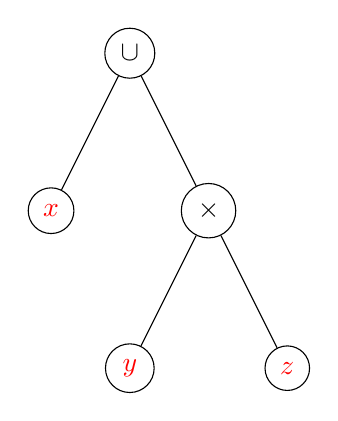
\begin{tikzpicture}[every node/.style={circle,draw,minimum size=5mm},level distance=2cm,
  level 1/.style={sibling distance=2cm},
  level 2/.style={sibling distance=2cm}
  ]
    
    \node {$\cup$}
        child { node {\textcolor{red}{$x$}}}  
        child{ node {$\times$}
                child { node {\textcolor{red}{$y$}} }
                child { node {\textcolor{red}{$z$}} }
        }
        ;
\end{tikzpicture}
    \caption{Possible vertex order in \Cref{Corollary 11}}
    \label{fig:Possible vertex orders in Remark 3}
    \end{subfigure}
    \qquad
    \begin{subfigure}[b]{0.49\textwidth}
    \centering
    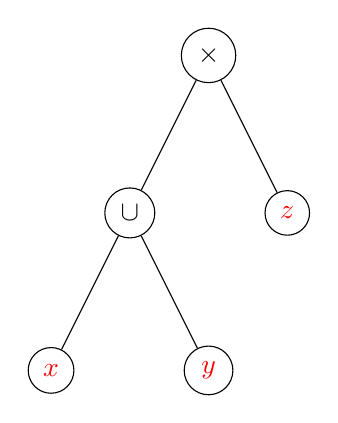
\begin{tikzpicture}[every node/.style={circle,draw,minimum size=5mm},level distance=2cm,
  level 1/.style={sibling distance=2cm},
  level 2/.style={sibling distance=2cm}
  ]
    
    \node {$\times$}
        child { node {$\cup$}
                child { node {\textcolor{red}{$x$} }}
                child { node {\textcolor{red}{$y$}} }
        }
        child{ node {\textcolor{red}{$z$}}}
        ;
\end{tikzpicture}



    \caption{Alternative vertex order in \Cref{Corollary 11}}
    \label{fig:Alternating vertex order in Remark 3}
    \end{subfigure}
    
    \label{fig:vertex orderings}
    \caption{Examples}
\end{figure}

Using \Cref{Ancestors remark}, we can uniquely determine the type of vertices for LCA of $x$ and $y$ and LCA of $y$ and $z$. If the LCA of vertices $x$ and $y$ is a descendant of the LCA of vertices $y$ and $z$, then the LCA of vertices $x$ and $y$ and the LCA of vertices $x$ and $z$ is the same vertex. The second case is considered similar. Both possible orders of the vertices are shown in the \Cref{fig:vertex orderings}.

\section{Partition}
All definitions below are taken from \cite{HABIB2005183}.
Let us introduce the critical concept of this section:
\begin{definition}[Partition]
  A \emph{partition} $P={X_1,\dots, X_k}$ of a set $V$ is a set of disjoint subsets of $V$ such that $X_1 \cup \dots \cup X_k=V$. We call ${X_1,\dots, X_k}$ the \emph{parts} of $P$.
\end{definition}

Let us denote a part containing vertex $x$ by $H_x$ \cite{HABIB2005183}.
 
\begin{definition}[Thinner relation]
Let $P$ and $Q$ be two partitions of $V$. If for each part $X$ of $P$ there exists a part $Y$ of $Q$ such that $X \subseteq Y$, then we say that $P$ is \emph{thinner} than $Q$ (or $Q$ is coarser than $P$).
\end{definition}

\begin{notation}
 Let $P$ be the partition $X_1,...,X_k$ of the set $V$.
Then we denote $X_i <_P X_j$ if and only if  $i<j$. And let $u \in X_i$ and $v \in X_j$ be any two arbitrary vertices from different parts. Then $u <_P v$ if and only if $i<j$.
\end{notation}

Let us define a partial order on the partitions of set $V$.
\begin{definition} [Compatibility]
    Let $P$ and $Q$ be two partitions of $V$, then $P$ is \emph{compatible} with $Q$, denoted by $P \leq Q$ if and only if both conditions hold:
    \begin{enumerate}
        \item $P$ is thinner than $Q$,
        \item for any $x$ and $y \in V$ such that $x <_P y$ it holds that $x \leq_Q y$.
    \end{enumerate}
\end{definition}

Additionally $P<Q$ if both $P \leq Q$ and $P \neq Q$.

\begin{definition}[Strict intersection, Definition 13 in \cite{HABIB2005183}]
    A set $S$ \emph{strictly intersects} another set $S_1$ if and only if $S \cap S_1 \neq \emptyset$ and the symmetric difference of sets $S$ and $S_1 \neq \emptyset$.
\end{definition}

\begin{definition}[Part refining]
 The \emph{refinement} of the part $H$ of the partition $P$ using a pivot set $S$ is replacing  part $H$ of the partition $P$ with two parts $H \cup S$ and $H - S$. 
\end{definition}

\begin{definition}[Partition refining]
 The \emph{refinement} of the partition $P$ using a pivot set $S$ is replacing each part $X_i$ of $P$ with two parts $X_i \cup S$ and $X_i - S$. The resulting partition after refinement is called Refine($P,S$).   
\end{definition}

In subsequent algorithms, the pivot set often denotes the set of neighbors of some vertex in the graph.
\begin{notation}[Pivot]
    If $S=N(x)$ where $N(x)$ is the neighborhood of vertex $x$, we call $x$ the \emph{pivot}.
\end{notation}

\begin{notation}[Splitter]
    If $N(x)$ strictly intersects $P$, we call vertex $x$ a \emph{splitter} of the partition $P$.
\end{notation}
 Note that a vertex $x$ is a splitter of $P$ if and only if $x$ separates at least two vertices within some part of $P$.

\section{Treewidth and pathwidth}
Treewidth and pathwidth are important structural parameters of graphs introduced in \cite{ROBERTSON1986309}.

A cotree $T$ can easily be transformed to an equivalent cotree $T_1$ such that every internal vertex in $T$ has exactly two sons. 
It holds from the associativity of the operation : $G=G_1 \times G_2 \times \dots \times G_k=G_1 \times (G_2 \times ( \dots \times(G_{k-1} \times G_{k} )\dots)$.


\begin{definition}[Definition 2.2 in \cite{Sumner1974DaceyG}]
    A tree-decomposition of a graph $G=(V,E)$ is a pair $(\{ X_i \colon i \in I\}$, $T=(I,F))$ with a family of subsets $\{ X_i \subseteq V \colon i \in I\}$, and a tree $T$, such that 
\begin{enumerate}
    \item $ \bigcup\limits_{i\in I} X_i=V$,
    \item There exists an appropriate $i \in I$ such that $v \in X_i $ and $w \in X_i$, for all $\{v,w\} \in E$,
    \item For all $v \in V$, each set $\{i \in I \colon v \in X_i \}$ induced a subtree of $T$.
\end{enumerate}
\end{definition}
Note that the third condition can be replaced by the following:
\begin{description}
    \item[$3'$]  For all $i, j, q \in I$ if $q$ is on the path from $i$ to $j$ in $T$, then $X_i \cap X_j \subseteq X_q$.
\end{description}



\begin{definition}[Treewidth, $tw(G)$]
The treewidth of a tree-decomposition $(\{X_i \colon\break i \in
I\}, T=(I,F))$ is defined as $\max\limits_{i\in I} |X_i|-1$.
The treewidth of $G$, tw($G$), is the minimum treewidth over all possible tree-decompositions of $G$.
\end{definition}


\begin{definition}[Definition 2.3 in \cite{Sumner1974DaceyG}]
    A path-decomposition of a graph $G=(V,E)$ is a pair $(\{ X_i \colon i \in I\}, I)$, with a family of subsets $\{ X_i \subseteq V \colon i \in I\}$, and there exists $r \in \mathbb{N}$ with $I=\{1,2,\dots,r\}$ such that
\begin{enumerate}
    \item $  \bigcup\limits_{i\in I} X_i=V$,
    \item There exists $i \in I$ such that $v \in X_i $ and $w \in X_i$, for all $\{v,w\} \in E$,
    \item There exists an appropriate $b_v, e_v \in \{1,2,\dots,r\}$, such that for all $v \in V$ and $i$ such that $v \in X_i$ it holds that $b_v \leq i \leq e_v$. And for all $i$ such that $b_v \leq i \leq e_v$ it holds that $v \in X_i$.
\end{enumerate}
\end{definition}

\begin{definition}[Pathwidth, $pw(G)$]
The pathwidth of $(\{ X_i \colon i \in I\}, I)$ is defined as $\max\limits_{i\in I} |X_i|-1$. The pathwidth of graph $G$, $pw(G)$, is the minimum pathwidth over all possible path-decompositions of $G$.
\end{definition}




